\documentclass[UTF8]{ctexart}

\usepackage[T1]{fontenc}
\usepackage{textcomp}
\usepackage{theorem}
\usepackage{bm}
% \usepackage[dutch]{babel}
\usepackage{amsmath, amssymb}
\usepackage{import}
\usepackage{pdfpages}
% \usepackage{transparent}
\usepackage{xcolor}
\usepackage{float}
% ------------- coding style setting --------------%
\usepackage{libertine}
\newfontfamily\cvtextfont[Path=/home/yujie6/Music/MATH/AbAlg/fonts/]{freebooterscript}
\newfontfamily{\FA}[Path=/home/yujie6/Music/MATH/AbAlg/fonts/]{FontAwesome}
\input{/home/yujie6/Music/MATH/AbAlg/fonts/fontawesomesymbols-xeluatex.tex}
\usepackage{listings}
\definecolor{codegreen}{rgb}{0,0.6,0}
\definecolor{codegray}{rgb}{0.5,0.5,0.5}
\definecolor{codepurple}{rgb}{0.58,0,0.82}
\definecolor{backcolour}{rgb}{0.95,0.95,0.92}

\lstdefinestyle{mystyle}{
    backgroundcolor=\color{backcolour},
    commentstyle=\color{codegreen},
    keywordstyle=\color{magenta},
    numberstyle=\tiny\color{codegray},
    stringstyle=\color{codepurple},
    basicstyle=\ttfamily\footnotesize,
    breakatwhitespace=false,
    breaklines=true,
    captionpos=b,
    keepspaces=true,
    numbers=left,
    numbersep=5pt,
    showspaces=false,
    showstringspaces=false,
    showtabs=false,
    tabsize=2
}

\lstset{style=mystyle}

% ----------------- geometry and fancy head -----------

\usepackage{geometry}
\geometry{left=2.5cm,right=2.5cm,top=3cm,bottom=3cm}
\usepackage[many]{tcolorbox}
\usepackage{fancyhdr}
\usepackage{syntonly} % dubugging
% \syntaxonly
\fancypagestyle{mainFancy}{
    \fancyhf{}
    %\renewcommand\headrulewidth{0pt}       % 页眉横线
    %\renewcommand\footrulewidth{0pt}
    
    \fancyhead[L]{RISC-V CPU}       % 页眉章标题
    \fancyhead[R]{Project Report}         % 页眉文章题目
    \fancyfoot[C]{\thepage}                 % 页眉编号
}
\pagestyle{mainFancy}


% --------------- environment setting ------------------

\newtheorem{thm}{Theorem}
\newtheorem{pro}{Problem}
\newtheorem{lemma}{Lemma}
\newtheorem{defi}{Definition}[section]
\newtheorem{li}{Example}[section]
\newenvironment{proof}{\paragraph{Proof:}}{\hfill$\square$}
\newenvironment{jie}{\paragraph{Show:}}{\hfill$\square$}
\tcolorboxenvironment{pro}{
  enhanced,
  borderline={0.4pt}{0.4pt}{black},
  boxrule=0.4pt,
  colback=white,
  coltitle=black,
  sharp corners,
}
\tcolorboxenvironment{thm}{
  enhanced,
  borderline={0.4pt}{0.4pt}{black},
  boxrule=0.4pt,
  colback=white,
  coltitle=black,
  sharp corners,
}

% ----------------- macros and command -----------------
\let\implies\Rightarrow
\let\impliedby\Leftarrow
\let\iff\Leftrightarrow
\let\ldots\cdots

\usepackage{stmaryrd}
\newcommand\contra{\scalebox{1.5}{$\lightning$}}
\definecolor{correct}{HTML}{009900}
\newcommand\correct[2]{\ensuremath{\:}{\color{red}{#1}}\ensuremath{\to }{\color{correct}{#2}}\ensuremath{\:}}
\newcommand\green[1]{{\color{correct}{#1}}}

% horizontal rule
\newcommand\hr{
    \noindent\rule[0.5ex]{\linewidth}{0.5pt}
}
\def\mf(#1){\mathfrak{#1}} 
\def\abs(#1){\left| #1 \right| }
\newcommand\setn[2]{\left\{#1_1,#1_2,\cdots, #1_#2 \right\}  }


\newcommand\dif{\,\mathrm{d}}
\newcommand\e{\,\mathrm{e}}
\newcommand\R{\,\mathbb{R}}
\newcommand\la{\,\lambda}
\newcommand\C{\,\mathbb{C}}
\newcommand\F{\,\varphi}
\newcommand\ep{\,\varepsilon}
\newcommand\N{\,\mathbb{N}}
\newcommand\Z{\,\mathbb{Z}}
\newcommand{\incfig}[2][0.3]{%
    \def\svgwidth{#1\columnwidth}
    \import{./figures/}{#2.pdf_tex}
}


\author{卢禹杰}

\title{\Huge\textsc{RISC-V CPU Project Report}}
\begin{document}
\maketitle
 
\section{简介}
本次大作业主要目的是实现一个基于RISCV架构, rv32ia指令集的CPU。本项目一共实现了以下内容:
\begin{itemize}
		\item 取指-译码-执行-访存-回写的五级流水架构
		\item FPGA 150MHz 测试通过
		\item 512Byte的指令缓存,可以容纳128条instruction,pi测试点时间为3s
\end{itemize}

本项目主要使用verilog硬件设计语言编写,使用iverilog进行模拟,Xilinx Vivado进行仿真综合。
(在写完大作业之后我才发现iverilog是一个很好的测试正确性的工具。我还写了一个脚本来进行快速测试正确性。)
\section{基本架构}
\begin{figure}[htpb]
		\centering
		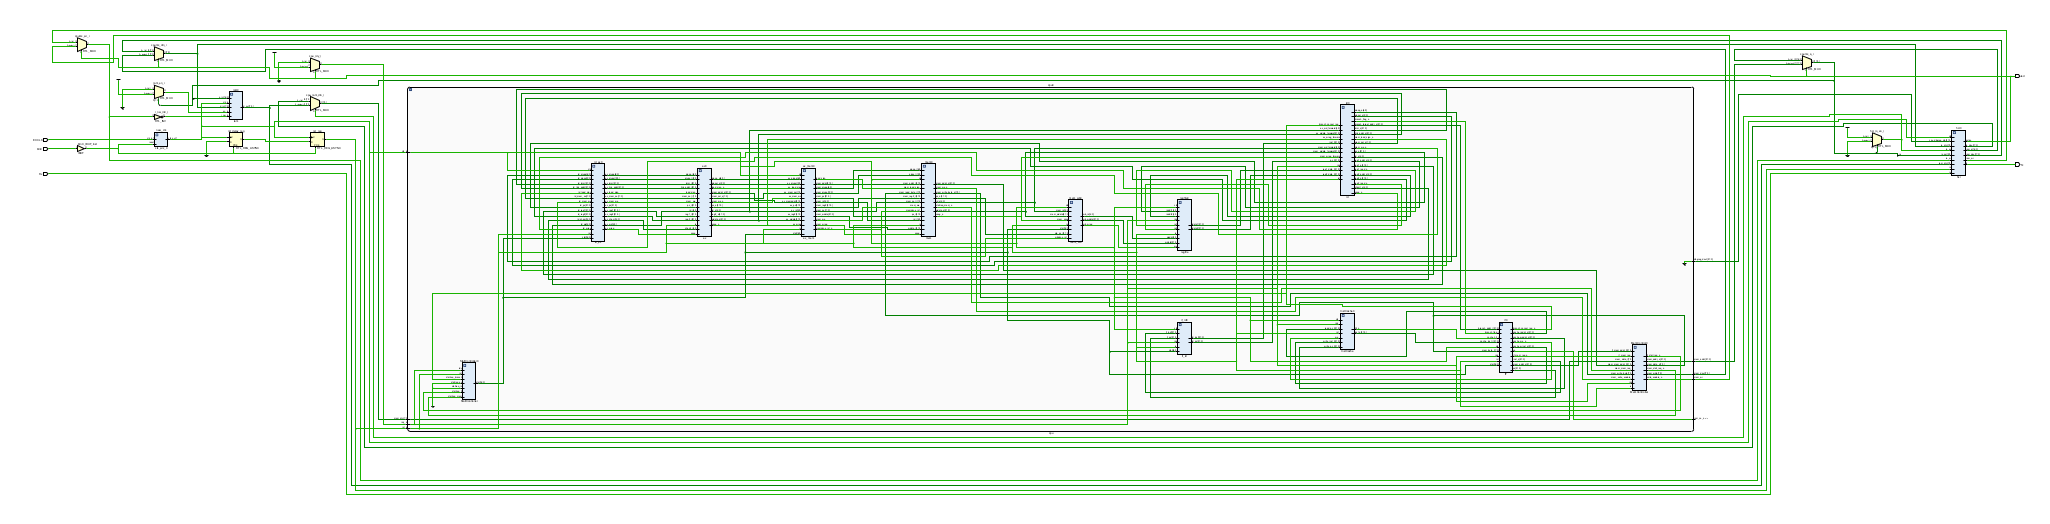
\includegraphics[width=0.8\textwidth]{arch.png}
		\caption{基本架构}
		\label{fig:arch-png}
\end{figure}
本项目采用的架构为经典的五级流水架构,cpu.v中各模块功能如下
\begin{enumerate}\setlength{\itemsep}{-0.06cm}
		\item if: 取指令模块,与MemoryController以及cache交互
		\item InstCache: 一个512 bytes的指令寄存器,可以做到hit两周期取值
		\item regfile: 寄存器模块,与wb和id交互
		\item if\_id: 流水线寄存器,将指令传给id
		\item id: 指令译码以及判断分支以及跳转与否
		\item id\_ex: 流水线寄存器,将指令以及译码信息传给ex
		\item ex: 指令执行,完成所有的计算工作
		\item ex\_mem: 流水线寄存器,将指令以及内存访问信息传给mem
		\item mem: 内存访问模块,与MemoryController交互
		\item mem\_wb: 流水线寄存器,将指令以及寄存器读写信息传给wb
		\item MemController: 调度取指令和mem阶段的内存访问,与真正的内存交互
		\item StallController: 控制流水线的暂停,解决hazard
\end{enumerate}
\section{遇到的问题}
在作业过程中,我主要遇到了一下问题
\begin{itemize}
		\item 安装RiscV Toolchain失败,之后我
				在官方社区提了issue并得到了解答,发现是大作业仓库上的的安装
				教程有问题。采用社区提供的安装教程我成功的安装上了,并且
				我写了一个更方便的脚本来生成.data文件。
		\item Linux上的Vivado有比较严重的bug,最开始我根本安装不上
				之后向社区提问之后我才知道是有两个动态链接库缺失了,
				手动创建软链接之后可以安装。之后Simulate的时候
				又出现了奇怪的报错,google之后也解决了这个问题。
		\item 最开始的时候不会取指令,感觉一个周期只能读一个字节实在是
				太麻烦了,之后看了学长的代码才想到用一个有限状态机来
				解决这个问题。
		\item 上板的时候我遇到了许多的critical warning。但是当我
				解决其中的两个warning之后,我发现自己的正确性又
				出大问题了,因为我有一个变量memdone必需在两个
				always语句中使用,尝试了很多方法都没解决。最后
				换了一个思路解决了这个问题。
\end{itemize}
\section{大作业心得}
本次大作业我学到了很多:
\begin{itemize}
		\item 对五级流水以及教材中的一些设计思想更加熟悉了。
		\item 学习了新的硬件设计语言,提升了自己的编程能力与设计能力。
		\item 对数字电路更加了解了。
\end{itemize}
\section{关于大作业的建议}
\begin{itemize}
		\item riscv-toolchain的安装教程需要更新,
				因为版本的错误浪费了很多时间在上面。
		\item 希望能够提供更多上板的教程和资料,很多时候错了不知道为什么,
				问了同学才知道。以及Vivado其实有一些很强大的功能,但我也是
				最后一周才从同学那里了解到的,希望以后能有更多的这方面的资料。
\end{itemize}


\end{document}
